\documentclass{ltjsarticle}
%\usepackage[dvipdfmx]{color}
\usepackage{booktabs}
\usepackage{mathcomp}
\usepackage{array}
\usepackage{mathtools,amssymb}
\usepackage{siunitx}
\usepackage{multirow}
\usepackage{tabularx}
\usepackage{subcaption}
\usepackage{float}
\usepackage{kcctd-report}
\usepackage{listings,jvlisting}
\lstset{
	basicstyle={\ttfamily},
	identifierstyle={\small},
	commentstyle={\smallitshape},
	keywordstyle={\small\bfseries},
	ndkeywordstyle={\small},
	stringstyle={\small\ttfamily},
	frame={tb},
	breaklines=true,
	columns=[l]{fullflexible},
	numbers=left,
	numberstyle={\scriptsize},
	stepnumber=1,
	lineskip=-05ex,
	tabsize=2
}
\renewcommand{\lstlistingname}{ソースコード}

\title{VHDLによるディジタル回路の設計(自由課題)}
\adviser{木場 隼介 先生}

\sdate{令和5年10月19日}
\edate{令和5年11月2日}
\fdate{令和5年11月7日}
\rdate{}

\grade{5}
\anumber{}
\gnumber{B}
\name{河合 将暉}
\jname{}
\comment{}
\begin{document}
\maketitle

\section{目的}
	自由課題を通してVHDLの構文規則や処理方法について詳しく知るとともに、
	プレゼンテーションを行い、課題に対する説明および発表能力を養うことを目的とする。
\section{自由課題}
	\subsection{仕様}
		本実験の自由課題のコンセプトとして、2人で対戦できるルーレットをFPGAで構成することを
		目標とした。仕様としては、FPGAデバッグボードに搭載されている10個のLEDのうち、
		左右から3個ずつのLEDを用いてルーレットを2組構成した。
		ルーレットのストップ・リセットにはFPGAボードに標準搭載されているタクトスイッチ4個を
		使用して1人あたりストップ・リセット用に2個スイッチを割り当てた。

		対戦のルールとして、ルーレットが揃う(LED3個が同色になる)と1点加点され、
		先に2点獲得したプレイヤーの勝利というようなルールを提案する。
		設計はこのルールをベースに設計を行ったが、ルール変更による拡張性にも視野に含めて
		設計した。
		対戦型ルーレットシステム稼働時のFPGAボードを図\refeq{fig:FPGA}に示す。
		\begin{figure}[H]
		\centering
		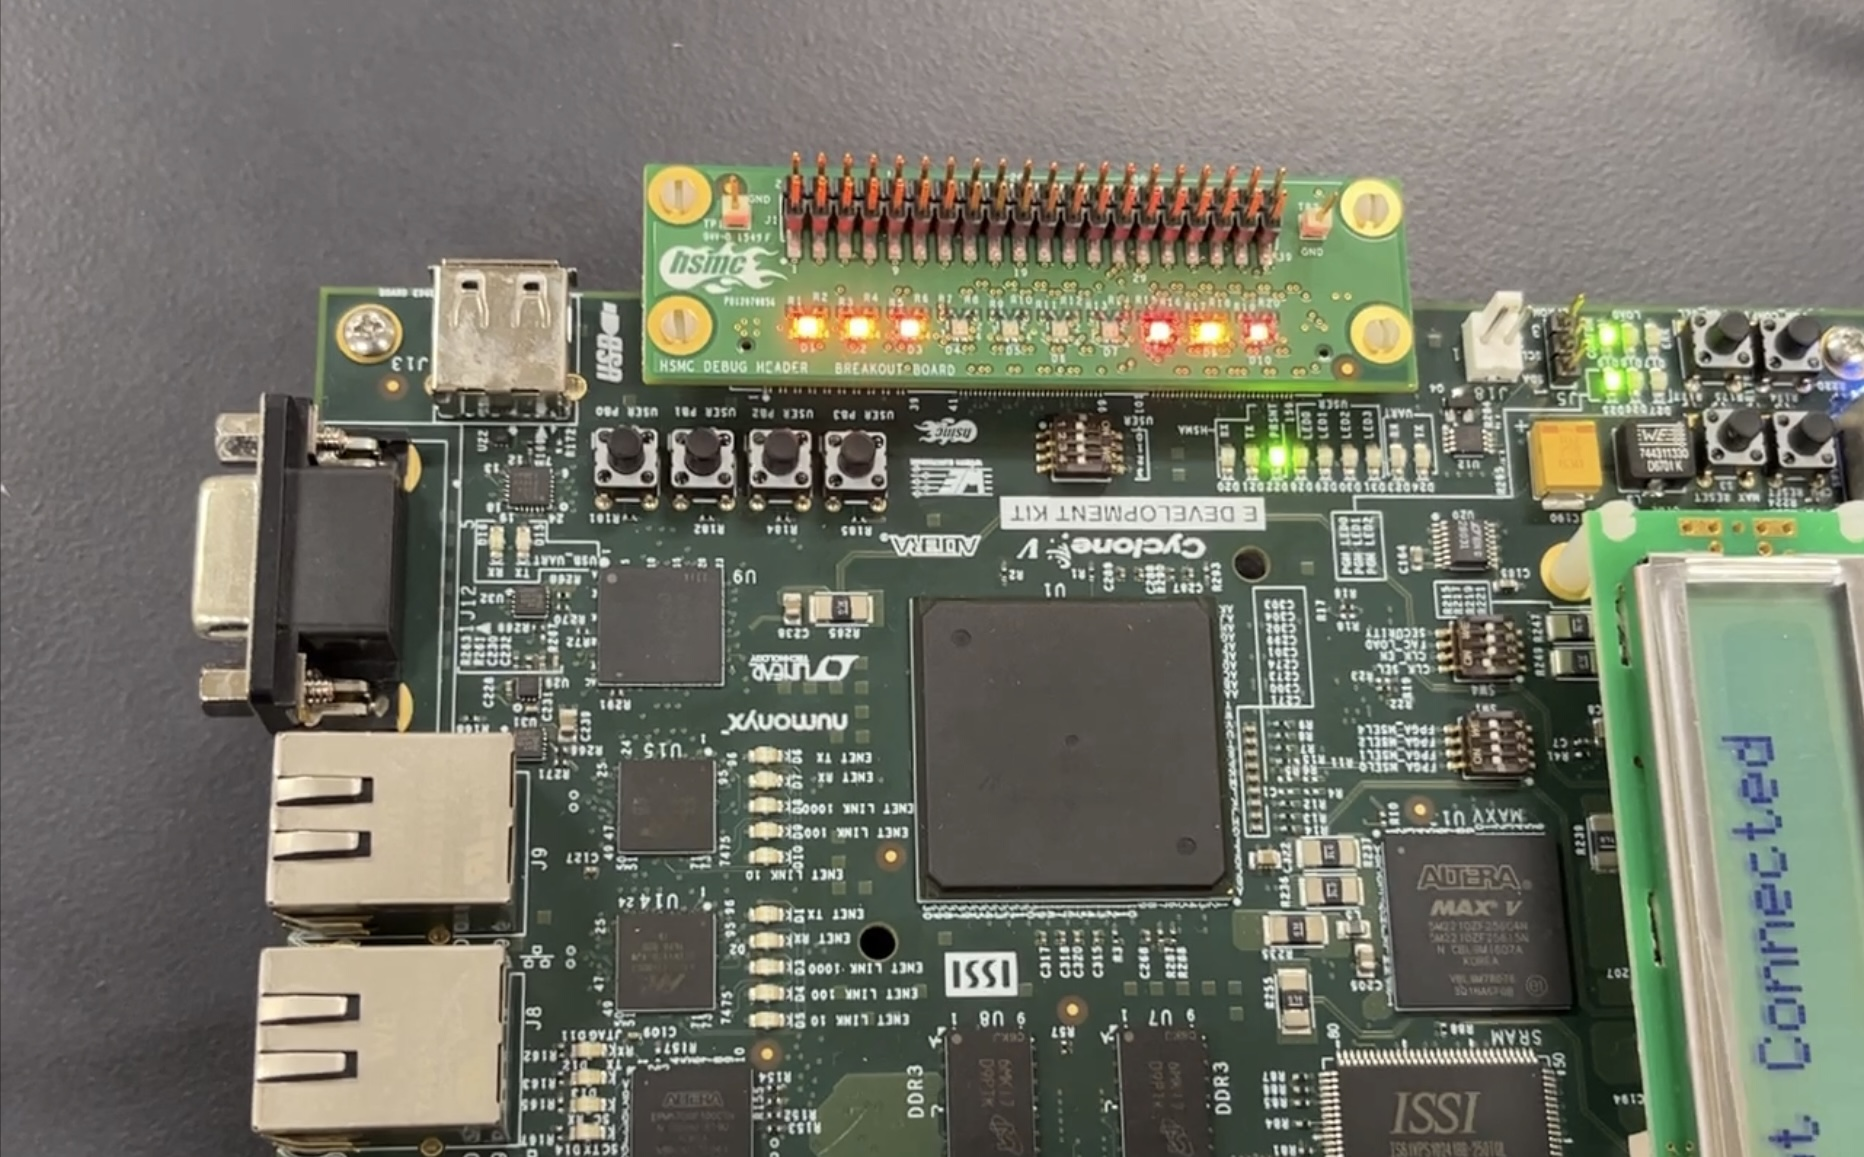
\includegraphics[width = 8cm]{figs/IMG_4552.PNG}
		\caption{FPGAボード上面図}
		\label{fig:FPGA}
		\end{figure}
	\subsection{参考にしたプログラム}
		自由課題の対戦型ルーレットシステムを構成する際に\cite{ref:指導書}のSample08vhdを参考に作成した。
		Sample08ではデバックボード上のLEDを3個、FPGAボード上のタクトスイッチを2個用いてルーレットを構成されていた。
		また、Sample08ではルーレット機能のみを記述したroulettevhdをポートとして呼び出し、マッピングを行ってルーレット機能を
		動作させていた。

	\subsection{使用器具}
		以下に、本課題で使用した器具を表\refeq{tab:used}に示す。
	\begin{table}[H]
	\begin{center}
	\caption{使用器具}
	\label{tab:used}
	\begin{tabular}{clllll} \toprule
	No&\multicolumn{1}{l}{機器名}&\multicolumn{1}{l}{型番}&\multicolumn{1}{l}{シリアルNo}&\multicolumn{1}{l}{備考}\\ \hline
	1&FPGAボード&Cyclone V E FPGA&2&シリアルNoは\\
	&&Development Kit&&外箱の番号を記載\\
	2&PC&ASUS TAF-Gaming&&\\
	\bottomrule
	\end{tabular}
	\end{center}
	\end{table}

\clearpage
\section{プログラム解説}
	\subsection{ピン割当}
		本課題でのデバッグボード上LEDのピン割当を表\refeq{tab:LEDpin}に示す。
		\begin{table}[H]
		\begin{center}
		\caption{デバッグボードLEDのピン割当}
		\label{tab:LEDpin}
		\begin{tabular}{cc|c} \toprule
			ピン名称&入出力&ピン番号\\ \hline
			led\_out0[0]&出力&PIN\_AF21\\
			led\_out0[1]&出力&PIN\_AJ20\\
			led\_out0[2]&出力&PIN\_AG22\\
			led\_out0[3]&出力&PIN\_AK20\\
			led\_out1[0]&出力&PIN\_AF20\\
			led\_out1[1]&出力&PIN\_AJ19\\
			led\_out1[2]&出力&PIN\_AG21\\
			led\_out1[3]&出力&PIN\_AK18\\
			led\_out2[0]&出力&PIN\_AF18\\
			led\_out2[1]&出力&PIN\_AJ17\\
			led\_out2[2]&出力&PIN\_AF19\\
			led\_out2[3]&出力&PIN\_AJ18\\
			led\_out3[0]&出力&PIN\_AG18\\
			led\_out3[1]&出力&PIN\_AG24\\
			led\_out3[2]&出力&PIN\_AG19\\
			led\_out3[3]&出力&PIN\_AH25\\
			led\_out4[0]&出力&PIN\_AK16\\
			led\_out4[1]&出力&PIN\_AH19\\
			led\_out4[2]&出力&PIN\_AK17\\
			led\_out4[3]&出力&PIN\_AH20\\
			led\_out5[0]&出力&PIN\_AF16\\
			led\_out5[1]&出力&PIN\_AG17\\
			led\_out5[2]&出力&PIN\_AG16\\
			led\_out5[3]&出力&PIN\_AH17\\
			led\_out6[0]&出力&PIN\_AE16\\
			led\_out6[1]&出力&PIN\_AJ15\\
			led\_out6[2]&出力&PIN\_AF15\\
			led\_out6[3]&出力&PIN\_AK15\\
			led\_out7[0]&出力&PIN\_AD17\\
			led\_out7[1]&出力&PIN\_AH14\\
			led\_out7[2]&出力&PIN\_AE17\\
			led\_out7[3]&出力&PIN\_AH15\\
			led\_out8[0]&出力&PIN\_AD18\\
			led\_out8[1]&出力&PIN\_AE15\\
			led\_out8[2]&出力&PIN\_AE18\\
			led\_out8[3]&出力&PIN\_AF14\\
			led\_out9[0]&出力&PIN\_Y15\\
			led\_out9[1]&出力&PIN\_AG23\\
			led\_out9[2]&出力&PIN\_AA15\\
			led\_out9[3]&出力&PIN\_AH22\\ \hline
		\end{tabular}
		\end{center}
		\end{table}

	本課題でのFPGAボード上スイッチのピン割当を表\refeq{tab:SWpin}に示す。
		\begin{table}[H]
		\begin{center}
		\caption{FPGAボードのピン割当}
		\label{tab:SWpin}
		\begin{tabular}{c|cc|c} \toprule
			部品名&ピン名称&入出力&ピン番号\\ \hline
			LED&led\_check1&出力&\\
			LED&led\_check2&出力&\\ \hline
			スイッチ&sw\_in1&入力&PIN\_AB12\\
			&sw\_in2&入力&PIN\_AG12\\
			&resetn1&入力&PIN\_AB13\\
			&resetn2&入力&PIN\_AF13\\ \hline
			クロック発振器&clk&入力&PIN\_P22\\
		\bottomrule
		\end{tabular}
		\end{center}
		\end{table}
	\subsection{実装した機能}
		\subsubsection{ルーレットの独立化}
			本課題で実装したシステムの独自性として、サンプルプログラムで構成されていたルーレットは
			1つのみであり、複数個を同時に動作させることは不可能であったが、本システムでそれを可能にした。
			単純にLEDを増設しただけではストップ・リセットの動作が全て同期したままであり、揃えるLEDが
			増えただけの大きなルーレットが構成されてしまう。
			これを解消するために、\cite{ref:指導書}から参照したサンプルプログラムのSample08vhdとroulettevhdを一部変更した。
			まず、Sample08におけるポート設定の変更箇所をソースコード\refeq{code:Sample08port}に示す。

			\begin{lstlisting}[caption = Sample08のポート設定, label = code:Sample08port]
			entity sample08 is
			generic (
				div_bits : integer := 15);
			
			port (
				clk     : in  std_logic;
				resetn1 : in  std_logic;
				resetn2 : in  std_logic;
				sw_in1  : in  std_logic;
				sw_in2  : in  std_logic;
				led_check1 : out std_logic :='1';
				led_check2 : out std_logic :='1';
				led_out0, led_out1, led_out2, led_out3, led_out4, led_out5 ,led_out6, led_out7, led_out8, led_out9 : out std_logic_vector(3 downto 0));

				end sample08;
			\end{lstlisting}

			ルーレット機能を複製するためにresetn,sw\_inを2つずつ用意し、led\_outを10個用意した。
			ルーレットを実装した段階ではled\_outは0〜2,7〜9の6個分しか使用していないが今後の
			システム拡張を想定し、デバッグボード上のすべてのLEDに割当を行った。

			次に、roulettevhdにおけるルーレット機能のポート設定をソースコード\refeq{code:roulettePort}示す。
			\begin{lstlisting}[caption = roulettevhd::ルーレット機能のポート設定, label = code:roulettePort]
			entity roulette is
			
			port (
				clk     : in  std_logic;
				resetn  : in  std_logic;
				sw_in1  : in  std_logic;
				sw_in2  : in  std_logic;
				led_out : out std_logic_vector(3 downto 0));

			end roulette;
			\end{lstlisting}
			サンプルプログラムでは、sw\_inは1個しかなかったため、2個用意し、どちらからの入力にもルーレットをストップさせる割当にした。

			Sample08でのルーレット機能のマッピングをソースコード\refeq{code:rouletteMap}に示す。
			\begin{lstlisting}[caption = Sample08vhd::ルーレット機能のマッピング, label = code:rouletteMap]
			component roulette
			
			port (
				clk     : in  std_logic;
				resetn : in  std_logic;
				sw_in1  : in  std_logic;
				sw_in2 : in  std_logic;
				led_out : out std_logic_vector(3 downto 0));

			end component;

			signal clk_div, clk_roulette, sw_node1, sw_node2 : std_logic := '0';
			signal div_counter : std_logic_vector(22 downto 0) := (others => '0');
			signal sw0, sw1, sw2, sw3, sw4, sw5, sw6, sw7, sw8, sw9: std_logic;
			signal sw_latch1, sw_latch_on1,sw_latch2, sw_latch_on2 : std_logic := '0';
			begin

			roulette_unit0 : roulette port map (
				clk     => clk_roulette,
				resetn   => resetn1,
				sw_in1   => sw0,
				sw_in2  => '0',
				led_out => led_out0);
			
			roulette_unit1 : roulette port map (
				clk     => clk_roulette,
				resetn   => resetn1,
				sw_in1   => sw1,
				sw_in2  => '0',
				led_out => led_out1);
			
			roulette_unit2 : roulette port map (
				clk     => clk_roulette,
				resetn   => resetn1,
				sw_in1   => sw2,
				sw_in2  => '0',
				led_out => led_out2);
			
			roulette_unit7 : roulette port map (
				clk     => clk_roulette,
				resetn   => resetn2,
				sw_in1  => '0',
				sw_in2   => sw7,
				led_out => led_out7);
			
			roulette_unit8 : roulette port map (
				clk     => clk_roulette,
				resetn   => resetn2,
				sw_in1  => '0',
				sw_in2   => sw8,
				led_out => led_out8);
				
			roulette_unit9 : roulette port map (
				clk     => clk_roulette,
				resetn   => resetn2,
				sw_in1  => '0',
				sw_in2   => sw9,
				led_out => led_out9);
			\end{lstlisting}

		roulette\_unit0〜2ではsw\_in1の入力に合わせてルーレットをストップさせるため、
		sw\_in1の入力をsw0〜2に代入した。また、sw\_in2の入力に影響を受けないように
		sw\_in2の入力を0にした。
		反対に、roulette\_unit7〜9ではsw\_in2の入力に合わせて代入を行い、sw\_in1の入力を0にした。

		ルーレットを止める機能のプログラムをソースコード\refeq{code:code:rouletteStop}に示す。
		\begin{lstlisting}[caption = sample08::ルーレットを止める機能,label = code:rouletteStop]
		  -- スイッチによるパルスを受け取ってルーレットを止めていく回路
		process (clk, resetn1,resetn2)
		begin  -- process
			if resetn1 = '0' then
			  sw0 <= '1';
			  sw1 <= '1';
			  sw2 <= '1';

			elsif clk'event and clk = '1' then  -- rising clock edge
			  if sw_latch1 = '1' then
			    if (sw0 = '1' and sw1 = '1' and sw2 = '1') then
			      sw0 <= '0';
			    elsif (sw0 = '0' and sw1 = '1' and sw2 = '1') then
			      sw1 <= '0';
			    elsif (sw0 = '0' and sw1 = '0' and sw2 = '1') then
			      sw2 <= '0';
			    end if;
			  end if;
			end if;
				
			if resetn2 = '0' then
			  sw7 <= '1';
			  sw8 <= '1';
			  sw9 <= '1';
			elsif clk'event and clk = '1' then  -- rising clock edge
			  if sw_latch2 = '1' then
			    if (sw7 = '1' and sw8 = '1' and sw9 = '1') then
			      sw7 <= '0';
			    elsif (sw7 = '0' and sw8 = '1' and sw9 = '1') then
			      sw8 <= '0';
			    elsif (sw7 = '0' and sw8 = '0' and sw9 = '1') then
			      sw9 <= '0';
			    end if;
			  end if;
		    end if;
		end process;
		\end{lstlisting}
		スイッチ入力(sw\_latch)が1になる場合,つまりスイッチ入力があったときに
		sw0~sw2に0を代入することによってLEDのルーレットをストップしている。
		sw7~sw9も同様の動作を行っている。
	\subsection{実装できなかった機能}
		\subsubsection{得点表示機能}
			本課題では2点先取のゲームを想定していたため,ルーレットが1回揃った段階でFPGAボード上のLED
			を点灯させ,現在の得点を表示する必要があると考えた。
			手法として,LED出力に用いているled\_outの値を参照して3つのLEDが同じ出力値の場合に
			FPGAボード上のLED出力をHIGHにして実装を試みたが,led\_outの値を参照して条件分岐
			をしようとすると変数型に関するエラーが出力された。
		
		\subsubsection{改善方法の検討}
			先述のエラーの原因は条件分岐として参照する値が出力型だったためと考えられる。
			改善するためにはポート設定をled\_out : out std\_logic\dots ではなく
			led\_out : buffer std\_logic\dots とすると入出力の両方で用いることができるため,
			エラーが出力されないと考えられる。
\section{質疑回答}
	\begin{itemize}
		\item 3人対戦は可能か\\
			現在構成しているシステムではFPGAボードに搭載されているスイッチの数が足りないため、不可能である。\\
		\item LEDを3個しか使用していない理由\\
			FPGAボード上で2人のプレイヤーがスイッチを押そうとすると相手の手で遮られて3個以上は見えづらいため
			ルーレットとしてある程度難しい3個で妥協している。\\
		\item プレイヤー表示を下のLEDの色分けで実装できないか\\
			FPGAボード上のLEDは単色LEDで緑色しか表示できないため、その方式では実装できない。
			デバックボード上ではLEDが4個余っているため、そのLEDを用いれば可能である。\\
		\item リセットボタンを用意するのではなくストップボタンの4回目でリセットにすればよいのではないか\\
			対戦人数を増やすという観点ではいい提案だと感じた。
			今回の課題の設計思想では、2人対戦をメインとしており、ユーザビリティの観点で
			ルーレットが揃わなかった際にボタンを数回連打するのと1回別のボタンを押すのでは
			別のボタンを押したほうがすぐにルーレットをやり直すことができてユーザビリティが
			高いと感じたため、ストップとリセットのスイッチを分けて実装した。\\
	\end{itemize}

\begin{thebibliography}{99}
\bibitem{ref:指導書}
「実験実習指導書『各種計算ハードウェアの活用〜VHDLによるディジタル回路の設計〜』」\\
神戸高専電子工学科 pp.28-36
\end{thebibliography}
\end{document}